\usetikzlibrary{patterns}
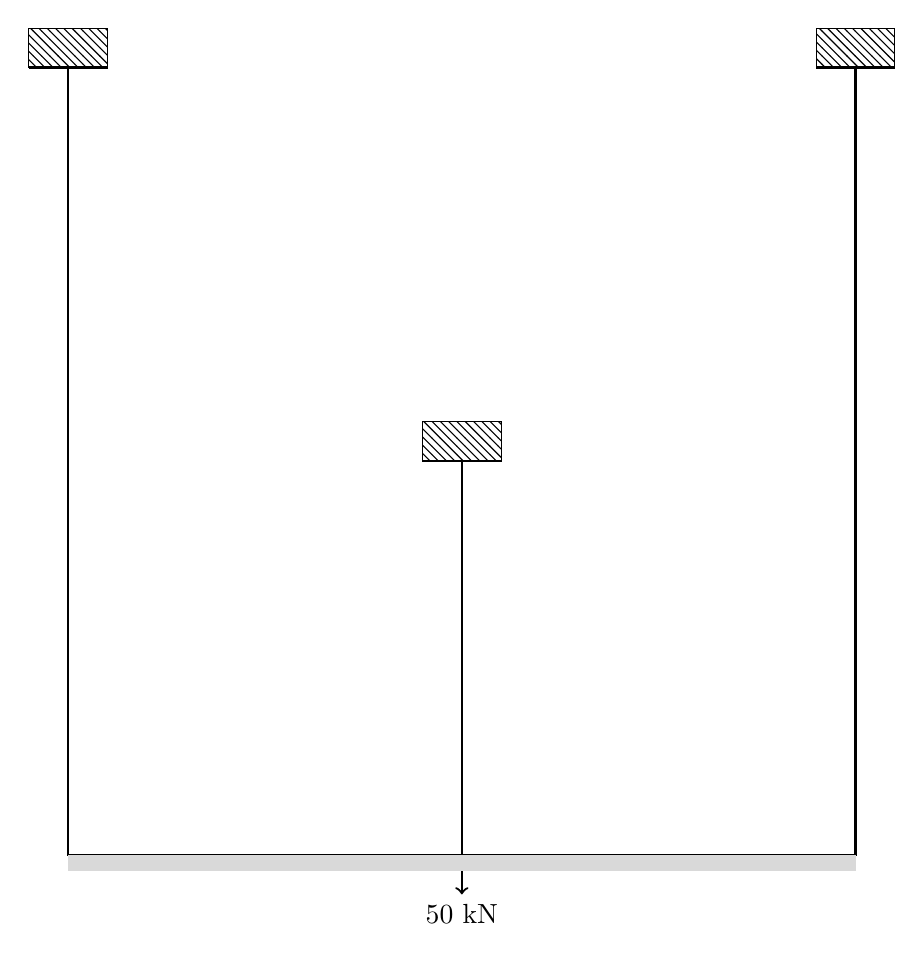
\begin{tikzpicture}

\draw[pattern = north west lines] (-0.5,0.5) rectangle (0.5,0);
\draw[pattern = north west lines] (9.5,0.5) rectangle (10.5,0);
\draw[pattern = north west lines] (4.5,-4.5) rectangle (5.5,-5);

\draw[thick] (-0.5,0) -- (0.5,0);
\draw[thick] (9.5,0) -- (10.5,0);
\draw[thick] (4.5,-5) -- (5.5,-5);

\draw[thick] (0,0) -- (0,-10) -- (10,-10) -- (10,0);
\draw[thick] (5,-5) -- (5,-10);
\draw[thin] (0,-10) -- (10,-10) -- (10,-10.2) -- (0,-10.2) -- (0,-10);

\draw[thick, ->] (5,-10.2) -- (5,-10.5) node[below] {50 kN};

\fill[gray!30] (0,-10) rectangle (10,-10.2);

\end{tikzpicture}
